La QKD (Quantum Key distribution), o Distribuzione Quantistica delle Chiavi, \`e una tecnologia di crittografia quantistica che permette la distribuzione di chiavi crittografiche con un livello di sicurezza inattacabile anche da computer quantistici. La QKD pu\`o essere suddivisa in due macro-classi DV-QKD e CV-QKD. Nella DV-QKD (Discrete-Variable Quantum Key Distribution) le informazioni vengono trasmesse utilizzando stati quantistici discreti, ad esempio la polarizzazione dei fotoni, che viene misurata attraverso apposite apparecchiature per ogni fotone. 

Il primo esempio di protocollo DV-QKD, come accennato nell'introduzione, \`e il BB84. In questo protocollo Alice trasmette sul canale quantistico a Bob una sequenza di fotoni polarizzati in modo casuale in due basi, ognuna delle quali ha due gradi di polarizzazione. Nella prima base il fotone pu\`o essere polarizzato a 0 o 90 gradi e verr\`a considerato come un bit 0, mentre nella seconda a 45 o 135 gradi e verr\`a considerato come bit 1.
In ricezione Bob effettuer\`a la misura della polarizzazione del fotone scegliendo una base con probabilit\`a uniforme dalle due basi disponibili. Alla fine della trasmissione Bob sar\`a in possesso dei gradi di polarizzazione misurati i quali verranno convertiti in 0 e 1 seguendo la stessa convenzione di Alice. Da notare che parte dei dati di Bob differir\`a da quelli inviati da Alice perch\`e Bob ha effettuato la misura utilizzando la base sbagliata.
Successivamente Bob comunicher\`a ad Alice quale base ha utilizzato per la misura di ogni fotone ed Alice scarter\`a tutti quei fotoni la cui base di trasmissione e misura non combaciano, e lo comunicher\`a a Bob. Fatto ci\`o Alice e Bob saranno in possesso, almeno in teoria, della stessa stringa random di bit.
Quello che potrebbe succedere \`e che durante la trasmissione Eve intercetti i fotoni inviati da Alice per effettuarne una misura e poi inviare il risultato della propria misura a Bob. Tuttavia questo altererebbe il risultato della misura di Bob perch\`e Eve non pu\`o sapere con quale base \`e stato polarizzato il fotone, e di conseguenza non pu\`o sapere con quale base misurarlo. Misurando un fotone con la base sbagliata nel momento in cui lo ritrasmetter\`a a Bob, egli ricever\`a un fotone polarizzato in modo differente rispetto a quello inviato da Alice. Questo permetter\`a ad Alice e Bob di determinare la presenza di una spia andando a confrontare una porzione di bit misurati con la stessa base utilizzata in trasmissione e quindi ritenuti uguali. Durante il confronto se si riscontrano bit diversi si determina la presenza di una spia. Se Eve ha intercettatto troppi fotoni non viene prodotta nessuna chiave e si ricomincia il protocollo da capo, in caso contrario si utilizzano i bit rimasti segreti come chiave crittografica\cite{zhao_development_2018}.

Nella CV-QKD (Continous-Variable Quantum Key Distribution), a differenza della DV-QKD per la trasmissione di informazioni vengono utilizzate variabili continue delle onde elettromagnatiche come ad esempio la fase.

In entrambe le classi di protocolli la sicurezza \'e garantita dai princ\'ipi delle fisica quantistica che ci permettono di rilevare eventuali intercettazioni da parte di Eve (spia) nella trasmissione su canale quantistico tra Alice (mittente) e Bob (destinatario).

La rilevazione \`e dovuta al fatto che durante la misura da parte di Eve lo stato quantistico viene alterato facendo diminuire l'energia del segnale se questo non viene amplificato~\footnote{Un'amplificazione, pur riportando il livello di energia del segnale a quello iniziale, introdurr\`a ulteriore rumore.} e introducendo del rumore, quindi dell'incertezza. All'atto pratico Eve intercetta lo stato coerente, rappresentato come in figura~\ref{fig:stato-coerente}, ne effettua una misura per poi ritrasmetterlo sul canale. Bob ricever\`a uno stato coerente con del rumore aggiunto e un minor numero di fotoni, ci\`o comporta che la gaussiana che lo rappresenta sar\`a caratterizzata da una varianza superiore a quella stimata e un valor medio pi\`u vicino allo zero. Per questo motivo, si effettuano numerosi run di trasmissione quantistica. In una fase preliminare si utilizza un certo numero di run per stimare i parametri di rumore del canale e, da essi, decidere se la trasmissione sta avvenendo in modo sicuro oppure no (si veda Sez.~\ref{subse:stima-parametri}). Nel caso in cui il controllo non vada a buon fine, la trasmissione corrente viene abortita perch\'e non \`e possibile garantire la sicurezza della chiave crittografica e si comincia con un nuovo round, se invece il controllo va a buon fine, il protocollo assicura che un'eventuale spia Eve non possa ottenere sufficiente informazioni sulla chiave condivisa fra Alice e Bob.

\section{CV-QKD con modulazione gaussiana}
Il protocollo di distribuzione quantistica di chiavi a variabili continue con modulazione gaussiana \`e un protocollo molto indicato per lo sviluppo e l'utilizzo su larga scala nel mondo reale data la sua affinit\`a con le infrastrutture oggi gi\`a esistenti, come ad esempio, i canali di comunicazione in fibra ottica. Come enunciato all'inizio del capitolo con questo protocollo si effettuano misure su variabili continue delle onde elettromagnetiche e in particolare nei protocolli con modulazione gaussiana gli stati coerenti da trasmettere sul canale di comunicazione vengono estratti da una distribuzione normale centrata in zero e una certa deviazione standard che viene definita in base ad alcuni fattori.

Il protocollo pu\`o essere suddiviso in due sezioni: la prima sezione ha effettivamente a che fare con segnali quantistici mentre la seconda sezione opera con segnali e dati classici. La prima sezione comprende la scelta e la trasmissione degli stati coerenti su fibra ottica da parte di Alice e termina nel momento in cui Bob effettua la misura; la seconda sezione comprende il sifting, la stima dei parametri e la riconciliazione.

\begin{figure}[H] 
\begin{center}
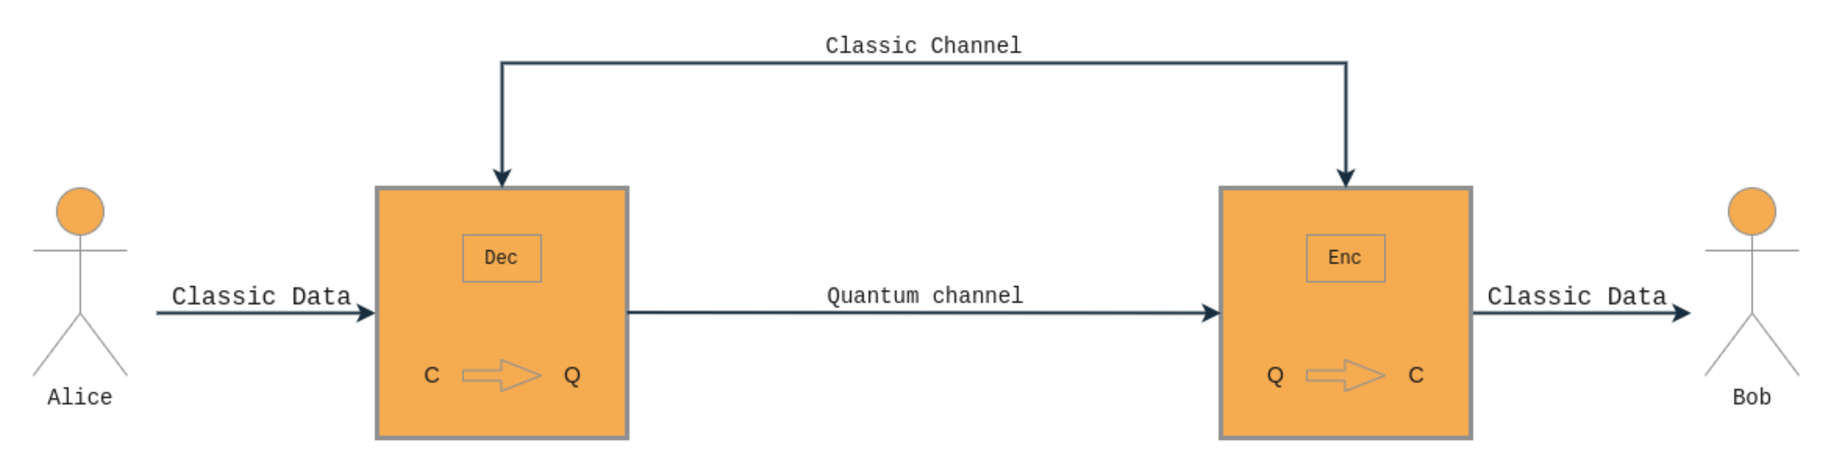
\includegraphics[width=\textwidth]{figure/alice_bob_communication.eps} 
\end{center}
\caption{Schema di comunicazione tra Alice e Bob Sezione.} \label{fig:alice-bob-schema}
\end{figure}

\subsection{Produzione, trasmissione e ricezione del segnale quantistico}\label{subse:sottosezione2-1-1}
Alice prepara gli stati coerenti andando a estrarre i valori delle componenti di quadratura $q$ e $p$ da una distribuzione normale centrata in zero ($q \sim {\mathcal N(0, V_{mod})}$ e $p \sim {\mathcal N(0, V_{mod})}$ )~\cite{https://doi.org/10.1002/qute.201800011}. Da notare che la distribuzione normale dalla quale Alice estrae le componenti di quadratura non ha nulla a che fare con le distribuzioni normali che caratterizzano gli stati coerenti ma rappresenta il modo in cui i dati vengono modulati. Dopo la preparazione Alice trasmette a Bob gli stati coerenti attraverso un canale di comunicazione, ad esempio una fibra ottica, che può essere anch'esso rappresentato come un canale quantistico.

Il canale \`e caratterizzato da un certo valore di trasmittanza $T$ e di rumore $\xi$. A causa della trasmittanza durante la trasmissione il segnale perde potenza quindi le gaussiane che descrivono lo stato coerente saranno centrate in un valore pi\`u vicino allo zero rispetto al momento della preparazione, mentre il rumore che viene introdotto fa aumentare la varianza delle gaussiane cos\`i da accrescere l'incertezza nelle misure da parte di Bob.

%da aggiungere le modifiche apportate dal professore
Per dare una rappresentazione matematica di quello che avviene ad uno stato coerente durante la trasmissione, possiamo andare a cosiderare un generico stato scelto da Alice $|\alpha_A \rangle = | q_A + i p_A\rangle$. Come abbiamo detto nella sezione~\ref{se:sezione1-1} le componenti di quadratura rispondono ad una distribuzione di probabili\`a normale. %quindi avremo:
%\begin{equation}
%\begin{split}
%Q_A \sim \mathcal N(q_A, 1) \\
%P_A \sim \mathcal N(p_A, 1)
%\end{split}
%\end{equation}
%In ricezione, a causa del canale, Bob andr\`a ad effettuare la misura su uno stato coerente alterato $|\alpha_B \rangle = | q_B + i p_B\rangle$ dove le componenti di quadratura rispondono alle seguenti distribuzioni gaussiane:
Bob andrà ad effettuare una misura su uno stato non più coerente, a causa della presenza di rumore ambientale. Tuttavia, lo stato quantistico ricevuto da Bob può ancora essere rappresentato utilizzando i valori medi di $\hat q$ e $\hat p$ e le loro varianze. Per lo stato ricevuto da Bob queste quantità prendono i seguenti valori:
\begin{equation}\label{eq:stato-bob}
\begin{split}
q_B = Mean(\hat{q}_B) = \sqrt{T} q_A, \quad Var(\hat{q}_B) &= 1 + \xi \\
p_B = Mean(\hat{p}_B) = \sqrt{T} p_A, \quad Var(\hat{p}_B) &= 1 + \xi 
%Var(q_B) &= 1 + \xi \\
%Var(p_B) &= 1 + \xi
\end{split}
\end{equation}
Pertanto, a tutti gli effetti, il canale ha come risultato quello di attenuare i valori medi e aumentare la varianza delle componenti di quadratura. 

Per la misura dello stato possono essere adottati due metodi diversi:
\begin{itemize}
\item \textbf{misura omodina}: Bob decide se misurare la componente di quadratura $q$ o $p$; la decisione viene presa attraverso una distribuzione di probabilit\`a uniforme. Per ciascuna componente di quadratura i valori misurati seguono le seguenti distribuzioni gaussiane:
\begin{equation}
\begin{split}
Q_B \sim \mathcal N(\sqrt{T}q_A, 1 + \xi) \\
P_B \sim \mathcal N(\sqrt{T}p_A, 1 + \xi)
\end{split}
\end{equation}
Per rimarcare quanto appenda detto, solo una delle due componenti verr\`a misurata.
\item \textbf{misura eterodina}: questa misura permette di misurare entrambe le componenti contemporaneamente, per\`o c'\`e un prezzo da pagare perch\'e effettuando questa misura viene aggiunto del rumore e la varianza delle distribuzioni normali ha un incremento di $1$. Anche i questo caso i valori misurati di entrambe le componenti seguono le seguenti distribuzioni di probabilit\`a gaussiane:
\begin{equation}
\begin{split}
Q_B \sim \mathcal N(\sqrt{T}q_A, 2 + \xi) \\
P_B \sim \mathcal N(\sqrt{T}p_A, 2 + \xi)
\end{split}
\end{equation}
\end{itemize}  

In caso di misura omodina \`e necessaria un'operazione addizionale cio\'e il sifting. Infatti, a questo punto del protocollo Alice \`e in posseso del doppio dei dati di Bob (in quanto Bob misura solo una della due componenti per ogni round) e per far s\`i che abbiano la stessa quantit\`a di dati correlati Bob rivela ad Alice, su canale classico pubblico, quale componente ha misurato ad ogni round; Alice prende nota della componenti misurate e scarta le altre\cite{milicevic_key_2018}. Notare che questa operazione non compromette la sicurezza: Eve saprà solo quale tipo di misura ha eseguito Bob ad ogni round, ma non il risultato ottenuto né il valore  vero inviato da Alice.

\subsection{Stima dei parametri}\label{subse:stima-parametri}
Dopo avere terminato la fase di trasmissione, Alice e Bob rivelano una porzione random di dati in modo tale da confrontare ci\`o che \`e stato effettivamente inviato da Alice con le misure di Bob. Da questo confronto sono in grado di stimare l'informazione mutua $I_{AB}$ (informazione mutua tra Alice e Bob) e l'informazione mutua tra Eve e Bob $\chi_{EB}$. Prima della effettiva stima delle mutue informazioni e necessario stimare trasmittanza e rumore del canale e calcolare altre quantit\`a che verranno utilizzare nel calcolo delle mutue informazioni.

Nel'articolo~\cite{https://doi.org/10.1002/qute.201800011} viene calcolata la segiente espressione per l'informazione mutua $I_{AB}$ \`e:
\begin{equation} \label{eq:AB-info}
I_{AB} = \frac{\mu}{2}\log_2(1 + SNR)
\end{equation}
con $\mu = 1$ se la misura \`e omodina e $\mu = 2$ per la misura eterodina. Qui la $SNR$ è la signal-to-noise ratio, data da::
\begin{equation} \label{eq:snr}
SNR = \frac{\frac{1}{\mu} T V_{mod}}{1 + \frac{1}{\mu} \xi}
\end{equation}

Per la stima di rumore e trasmittanza del canale abbiamo bisogno dei parametri $a$, $b$ e $c$ che rappresentano le entry della matrice di covarianza $\Sigma_{AB}$. Tale matrice rappresenta la covarianza fra le quadrature $\hat q$ e $\hat p$ per lo stato quantistico e deve essere stimata a partire dai risultati delle misure di Bob.
\begin{equation}
\Sigma_{AB} =
\begin{pmatrix}
a \mathbb{1}_2 & c \mathbb{1}_2 \\
c \mathbb{1}_2 & b \mathbb{1}_2
\end{pmatrix}
\end{equation}

Le equazioni per il calcolo dei parametri vengono ancora una volta prese dai risultati dell'articolo~\cite{https://doi.org/10.1002/qute.201800011}:
\begin{equation}
\begin{split}
a& = V_{mod} + 1 \\
b& = \frac{\langle q_B^2 \rangle + \langle p_B^2 \rangle}{2} \\
c& = \sqrt{\frac{V_{mod} + 2}{V_{mod}}} \cdot \biggl ( \frac{\langle q_Aq_B \rangle + \langle p_Ap_B \rangle}{2}\biggr )
\end{split}
\end{equation}

Calcolati i parametri $a$, $b$ e $c$ possiamo andare a stimare il rumore e la trasmittanza:
\begin{equation}
\begin{split}
T& = \frac{c^2}{V_{mod}^2 + 2V_{mod}} \\
\xi& = b - TV_{mod} -1
\end{split}
\end{equation}

Ora non ci resta che calcolare $\chi_{EB}$ in questo modo \ref{https://doi.org/10.1002/qute.201800011}:
%Ora non ci resta che calcolare le quantit\`a $\nu_1$, $\nu_2$ e $\nu_3$ alle quali verr\`a applicata una funzione $g(\nu)$ che ci porter\`a al calcolo della mutua informazione fra Eve e Bob. Finalmente \`e giunto in momento di calcolare anche $\chi_{EB}$ in questo modo:
\begin{equation} \label{eq:EB-info}
\chi_{EB} = g(\nu_1) + g(\nu_2) - g(\nu_3)
\end{equation}
Per fare questo avremo bisogno dei valori delle quantit\`a $\nu_1$, $\nu_2$ e $\nu_3$ che possiamo calcolare come segue:
\begin{equation} \label{eq:nuCalc}
\begin{split}
\nu_1& = \frac{1}{2}[z + (b - a)] \\
\nu_2& = \frac{1}{2}[z - (b - a)] \\
\nu_3& = \sqrt{a (a - \frac{c^2}{b})}
\end{split}
\end{equation}
con $z = \sqrt{(a + b)^2 - 4 c^2}$.

La funzione $g(\nu)$ per il calcolo di della mutua informazione fra Eve e Bob \`e definita in questo modo:
\begin{equation} \label{eq:g}
g(\nu) = \Bigl (\frac{\nu + 1}{2}\Bigr ) \log_2 \Bigl (\frac{\nu + 1}{2}\Bigr ) - \Bigl (\frac{\nu - 1}{2}\Bigr ) \log_2 \Bigl (\frac{\nu - 1}{2}\Bigr )
\end{equation}

Infine, dopo aver calcolato l'informazione mutua tra Alice e Bob e quella tra Eve e Bob vengono confrontati i risultati e nel caso in cui $\chi_{EB}$ risulti essere maggiore di $\beta I_{AB}$ \footnote{$\beta$ rappresenta l'accuratezza nel processare i dati dopo la trasmissione e viene calcolata come il rapporto tra il code-rate del codice classico scelto e la mutua informazione tra Alice e Bob} il protocollo viene abortito.

\subsection{Riconciliazione delle informazioni}\label{subse:riconciliazione}
Se la stima dei parametri ha avuto successo Alice e Bob sono in possesso di due stringhe di numeri reali diversi ma correlati, a causa degli errori introdotti durante la trasmissione sul canale e la misurazione di Bob. Devono pertanto effettuare una riconciliazione fra queste due stringhe, per assicurarsi di ottenere una sola stringa condivisa da entrambi. La riconciliazione pu\`o avvenire in due forme: 

\begin{itemize}
\item \textbf{diretta}: Alice produce un messaggio fittizio codificando i suoi dati (correlati a quelli di Bob) con una chiave. Bob basandosi sulle misure effettuate in fase di trasmissione cerca di estrarre la chiave dal messaggio fittizio;
\item \textbf{inversa}: la procedura \`e la stessa della riconciliazione diretta solamente che vengono scambiate le parti, Bob produce il messaggio fittizio ed Alice cerca di estrarre la chiave.
\end{itemize} 

Le due procedure differiscono nella scelta di quali sono i dati primari: nella riconciliazione diretta i dati di Alice sono i dati primari e Bob corregge i suoi dati di conseguenza, mentre nella riconciliazione inversa sono i dati di Bob ad essere primari, vengono inviati ad Alice la quale li utilizza per correggere i propri dati. 
 
La riconciliazione diretta presenta un problema: non pu\`o essere utilizzata per valori di trasmittanza troppo bassi, questo perch\'e Eve avrebbe pi\'u informazione sui dati di Alice rispetto a Bob e quindi risulterebbe impossibile creare una chiave crittografica sicura. D'altro canto la riconciliazione inversa non presenta questo problema quindi \`e possibile utilizzarla anche con valori bassi di trasmittanza, per\`o \`e da tenere in considerazione che pi\`u bassa \`e la trasmittanza pi\`u sar\`a distruttivo l'effetto del rumore del canale~\cite{https://doi.org/10.1002/qute.201800011}.

%Prima della riconciliazione vera a propria i dati in possesso ad Alice e Bob vengono normalizzati in modo tale da ottenere dei dati correlati. Se chiamiamo $\textbf{X}$ i dati in possesso ad Alice e $\textbf{Y}$ i dati in possesso a Bob, la relazione fra questi dati sar\`a $\textbf{X} = \textbf{Y} + \textbf{Z}$, dove $\textbf{Z}$ \`e una variabile aleatoria che risponde ad una distribuzione normale certata in zero con varianza $\frac{1}{V_{mod}}$. Attraverso questa normalizzazione in pratica, si ottiene lo stesso risultato che avremmo ottenuto se avessimo inviato ad Alice i dati di Bob attareverso una canale classico che aggiunge solamente rumore gaussiano.

A questo punto del protocollo Alice e Bob sono in possesso del subset di dati non utilizzati per la stima dei parametri che andiamo a chiamare $\textbf{X}_0$ e $\textbf{Y}_0$; prima di effettuare la riconciliazione vengono prodotte, a partire dai dati in loro possesso, altre due sequenze di dati correlati. 

Quello che ci aspettiamo \`e che le varianze dei dati in possesso di Alice e Bob siano rispettivamente:
\begin{equation}
\begin{split}
V_{X_0} &= V_{mod} + 1 \\
V_{Y_0} &= T V_{mod} + 1 + \xi
\end{split}
\end{equation}
Detto questo possiamo normalizzare $\textbf{X}_0$ e $\textbf{Y}_0$ in questo modo:
\begin{equation}\label{eq:normalizzazione}
\begin{split}
\textbf{X} &= \frac{\textbf{X}_0}{\sqrt{V_{mod}}}\\
\textbf{Y} &= \frac{\textbf{Y}_0}{\sqrt{T V_{mod} + 1 + \xi}}
\end{split}
\end{equation}
Cos\`i facendo abbiamo ottenuto altre due sequenze di dati $\textbf{X}$ e $\textbf{Y}$, correlate tra loro dall'equazione $\textbf{X} = \textbf{Y} + \textbf{Z}$, dove $\textbf{Z}$ \`e una variabile aleatoria che risponde ad una distribuzione normale centrata in zero e con varianza $V_z = \frac{1}{V_{mod}}$. Quindi normalizzando in questo modo abbiamo ottenuto lo stesso effetto che avremmo avuto se Bob avesso inviato ad Alice i proprio dati normalizzati $\textbf{Y}$ su un canale classico e pubblico che aggiunge solamente rumore gaussiano\cite{milicevic_key_2018}. Questo è il prototipo di canale di comunicazione classico utilizzato sin dai tempi di Shannon, detto canale di rumore bianco gaussiano additivo - Additive White Gaussian Noise Channel (AWGN). Per la trasmissione dati sull'AWGN è quindi possibile sfruttare una vasta gamma di codici studiati a partire dagli anni '60~\cite{Gallager_1972}-\cite{richardson2008modern}. 

Il passo successivo per Bob sar\`a quello di generare una stringa di bit random $\textbf{s} \in \{0,1\}^k$. Attraverso algoritmi di codifica LDPC (Low-Density Parity-Check)~\cite{borwankar_low_nodate} viene calcolata una matrice \textbf{H} necessaria per aggiungere alla stringa \textbf{s} dei bit ridondanti di parit\`a ottenendo la stringa $\textbf{c} \in \{0,1\}^n$ dove $n$ corrisponde alla lunghezza della sottosequenza di dati non utilizzati per la stima dei parametri.

I LDPC~\cite{borwankar_low_nodate} che rappresentano una classe di codici correttori di errori utilizzari nell'ambito delle telecomunicazioni. Una delle ragioni per cui questi codici sono largamente utilizzati \`e la loro abilit\`a di raggiungere prestazione vicine alla capacit\`a teorica del canale di comunicazione, nota come il limite di Shannon. I codici LDPC possono essere rappresentati in due modi:
\begin{itemize}
\item come una matrice di dimensioni $M \times N$ dove $N$ rappresenta la dimensione del messaggio che si vuole codificare ed $M = N - k$, con $k$ ottenuto dal prodotto tra $N$ e il code-rate, corrisponde al numero di bit ridondanti nel messaggio codificato, che vengono utilizzati per la correzione degli errori. Questa matrice \`e prevalentemente composta da zeri e contiene un numero limitato di uno.
\item come una grafo bipartito rappresentato da nodi check e nodi variabile; facendo riferimento alla rappresentazione matriciale il numero di nodi check \`e $M$ (numero di righe della matrice) e quello di nodi variabile \`e $N$ (numero di colonne della matrice). Gli uno contenuti nella matrice, nel grafo, sono denotati dagli archi che collegano un nodo variabile ad un nodo check.
\begin{figure}[H] 
\begin{center}
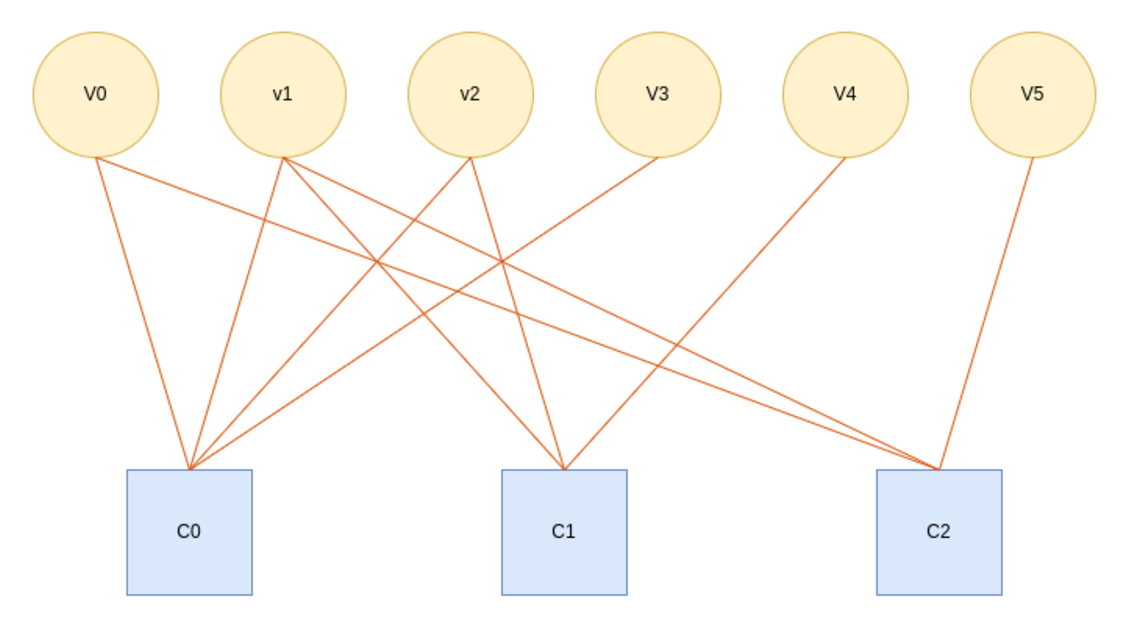
\includegraphics[width=0.8\textwidth]{figure/tanner_graph.eps} 
\end{center}
\caption[Grafo bipartito]{Grafo bipartito che rappresenta la matrice di parit\`a, in questo particolare caso fa riferimento alla matrice H \ref{eq:h-matrix} sottostante.}
\end{figure}
\end{itemize}

Attraverso gli algoritmi LDPC viene calcolata una matrice \textbf{H} che sar\`a della forma $\bigl [ -P^T_{(M \times k)} | I_{N-k}\bigr ]$:
\begin{equation} \label{eq:h-matrix}
\textbf{H} =
\begin{pmatrix}
 1 & 1 & 1 & 1 & 0 & 0 \\
 0 & 1 & 1 & 0 & 1 & 0 \\
 1 & 1 & 0 & 0 & 0 & 1
\end{pmatrix}
\end{equation}
\captionof*{mat}{Esempio di una matrice con $M=3$ ed $N=6$.}

Dalla matrice \textbf{H} possiamo ottenere la matrice generatore $\textbf{G} = \bigl [  I_{k} | P_{(k \times M)} \bigr ]$ da una matrice identit\`a di dimensione $k$ e la trasposta della matrice $P^T_{(M \times k)}$ :
\begin{equation}
\textbf{G} =
\begin{pmatrix}
 1 & 0 & 0 & 1 & 0 & 1 \\
 0 & 1 & 0 & 1 & 1 & 1 \\
 0 & 0 & 1 & 1 & 1 & 0
\end{pmatrix}
\end{equation}

Successivamente tramite il prodotto matriciale $\textbf{s} \times \textbf{G}$ tra la stringa \textbf{s} e la matrice generatore \textbf{G} si ottiene la stringa \textbf{c} che verr\`a utilizzata per modulare il segno della sequenza \textbf{Y} ottenedo cos\`i un nuovo messaggio \textbf{m} tale che $m_i = Y_i(-1)^{c_i}$ per $i = 1,2,\dots,n$.

%Il messaggio \textbf{m} viene trasmesso ad Alice su canale classico publico che assumiamo non introduca errori. Alice estrae da \textbf{m} un messaggio fittizio \textbf{r} con $r_i = \frac{m_i}{X_i}$ che corrisponde alla trasmisione su un canale Gaussiano con rumore di varianza $V_i = \frac{V_z}{|X_i|}$.

%Per tutti gli elementi del messaggio \textbf{r} vengono calcolati i valori di varianza che a loro volta vengono utilizzati per calcolare le LLRs (log-likelihood ratios) che sono definite come~\cite{gumucs2021novel}:
%\begin{equation}
%l_i = \log \frac{P(R_i = r_i| C_i = 0)}{P(R_i = r_i| C_i = 1)} = \frac{2r_i}{V_i}
%\end{equation}

%Le LLRs sono il logaritmo del rapporto tra la probabilit\`a condizionata che il messaggio $r_i$ provenisse effettivamente da un bit $0$ e la probabilit\'a che il messaggio $r_i$ provenisse da una bit $1$. I valori di LLRs permettono ad Alice, grazie all'utilizzo di un algoritmo LDPC di decodifica~\ref{al:sum-prod}, di ottenere una stima $\textbf{c'}$ della stringa $\textbf c$ prodotta da Bob.

Il messaggio \textbf{m} viene trasmesso ad Alice su canale classico publico che assumiamo non introduca errori. Alice estrae da \textbf{m} un messaggio fittizio \textbf{r} che le permettar\`a, attraverso l'utilizzo dell'algoritmo $\textit{sum-product}$~\ref{al:sum-prod}, di ottenere una stima della stringa di bit $\textbf{c}$ prodotta originariamente da Bob.

\section{Discussione della sicurezza contro attacchi di lettura del segnale}
Questo protocollo \`e particolarmente sicuro perch\'e consente il rilevamento di un'eventuale spia (Eve). Nel protocollo si assume che Eve sia in possesso di un computer quantistico e che abbia accesso completo al canale di comunicazione ed anche con queste assunzioni si \`e in grado di garantire la sicurezza per diversi tipi di attacchi.

Gli attacchi presi in considerazione tipicamente sono tre e differiscono per la loro efficacia:
\begin{itemize}
\item \textbf{attacchi individuali}: Eve effettua operazioni singolarmente su ogni segnale che viene scambiato tra Alice e Bob. 
\begin{figure}[H] 
\begin{center}
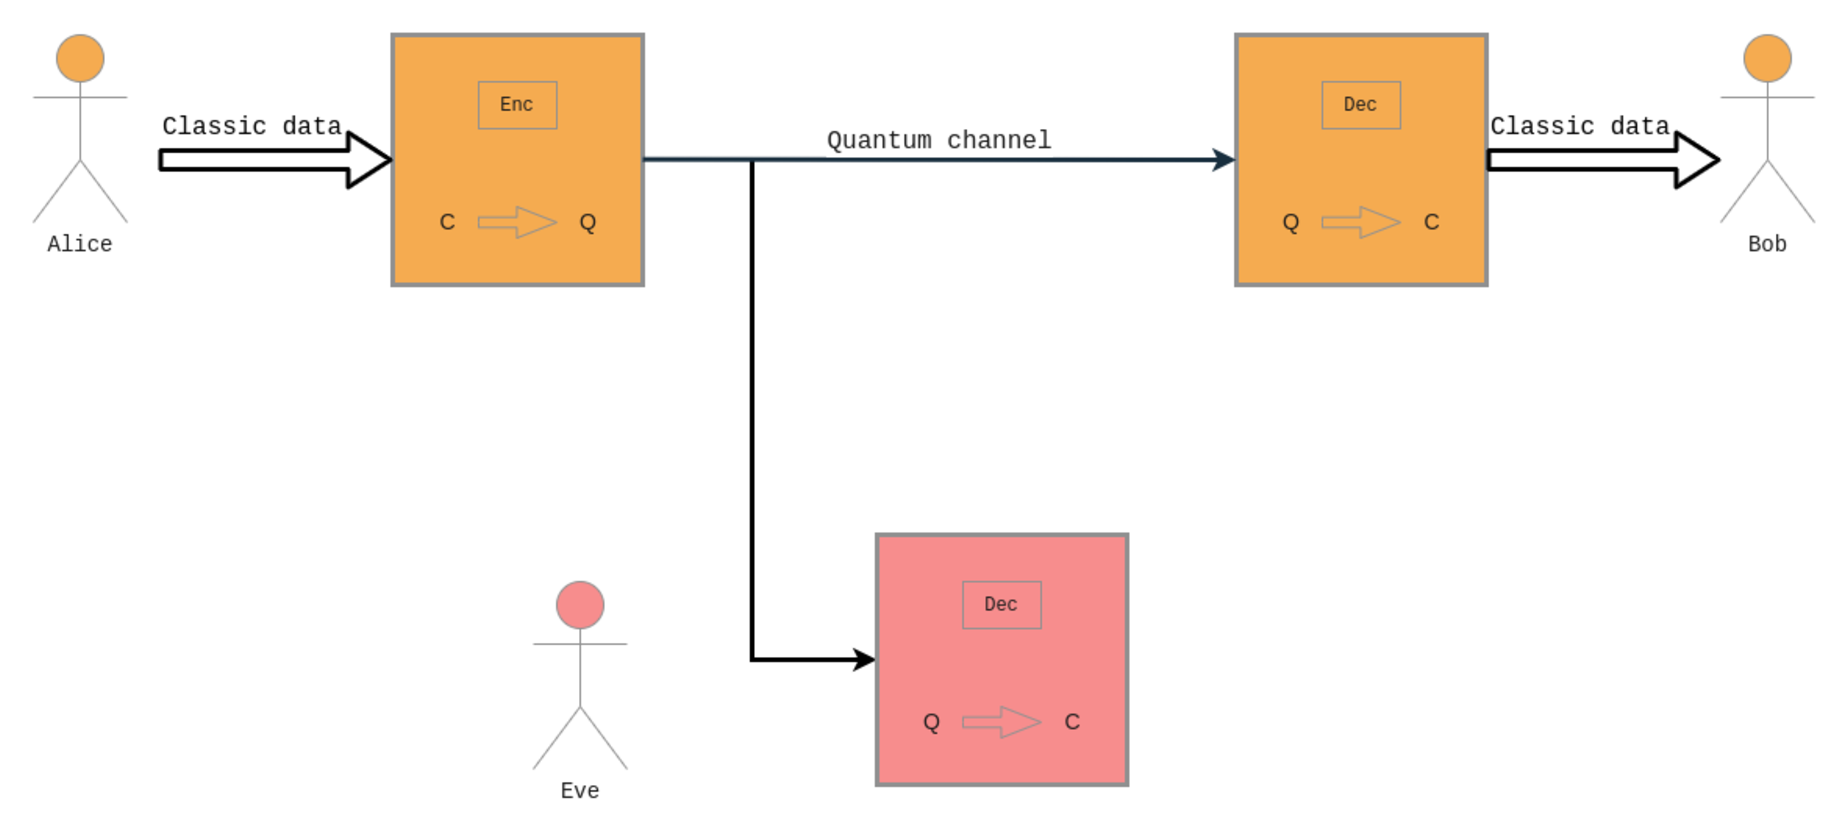
\includegraphics[width=0.8\textwidth]{figure/individual_attack.eps} 
\end{center}
\caption[Schema attacco individuale]{Schema che descrive un attacco individuale ponendo attenzione nel mostrare che le operazioni da parte di Eve vengono svolte singolarmente su ogni segnale.} \label{fig:attacco-individuale}
\end{figure}
\item \textbf{attacchi collettivi}: Eve salva nella memoria del suo computer quantistico un certo numero di stati sui quali effettua una misura collettiva. Questo attacco \`e pi\`u potente del precedente perch\`e secondo i pricipi della fisica quantistica effettuando una misura collettiva si pu\`o potenzialmente ricavare pi\`u informazione che dalla misura del singolo stato.
\begin{figure}[H] 
\begin{center}
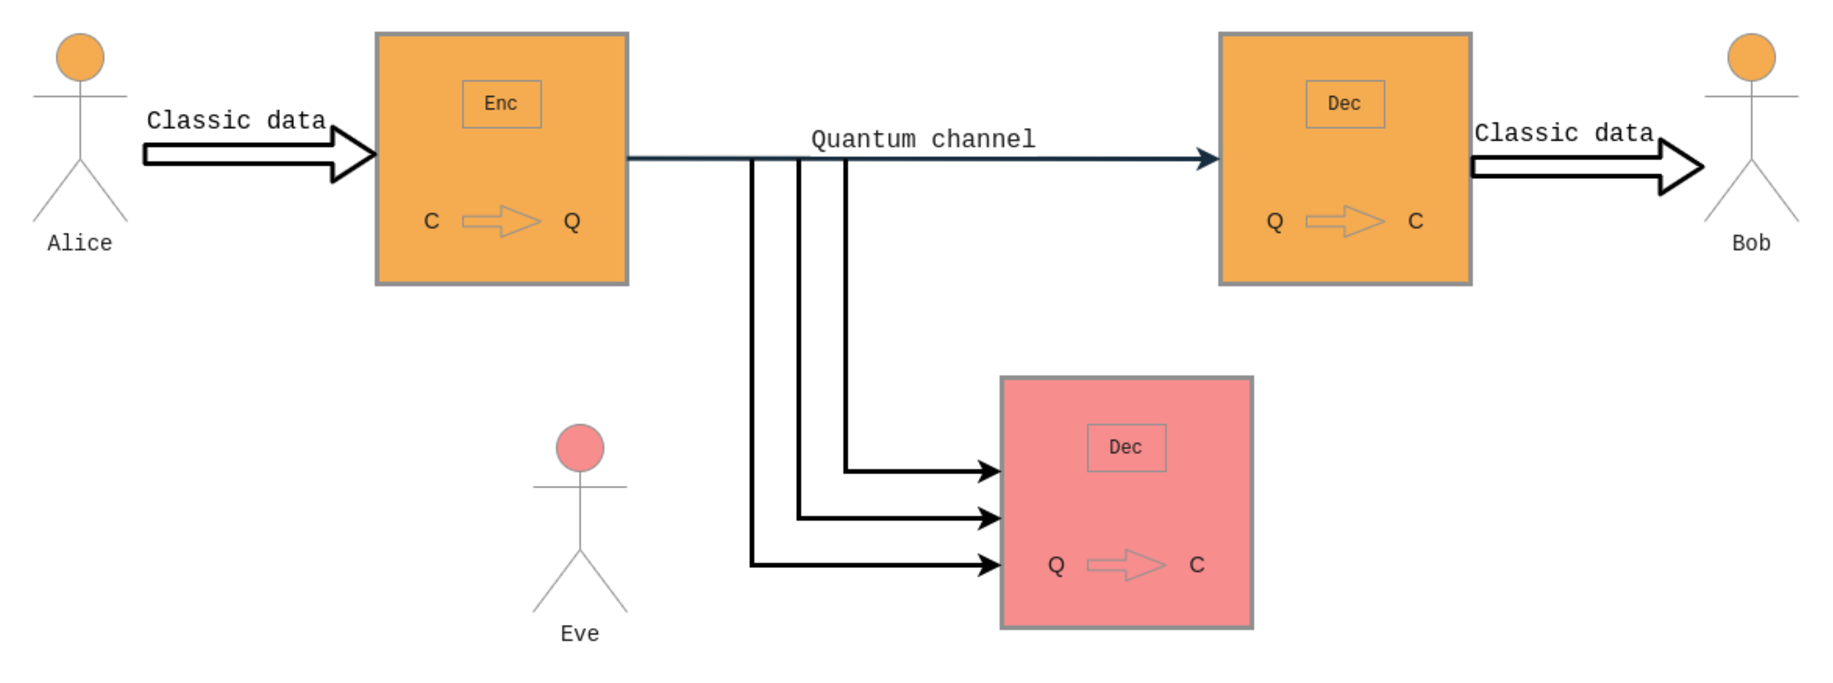
\includegraphics[width=0.8\textwidth]{figure/collective_attack.eps} 
\end{center}
\caption[Schema attacco collettivo]{Schema che descrive un attatto collettivo mostrando che Eve effettua operazione su pi\`u segnali contemporaneamente.} \label{fig:attacco-collettivo}
\end{figure}
\item \textbf{attacchi coerenti}: sono attacchi pi\`u potenti dei collettivi perché Eve, oltre alla lettura collettiva, può utilizzare delle correlazioni quantistiche, cioé entanglement, per mettere in relazione gli stati di pi\`u run.
%\begin{figure}[H] 
%\begin{center}
%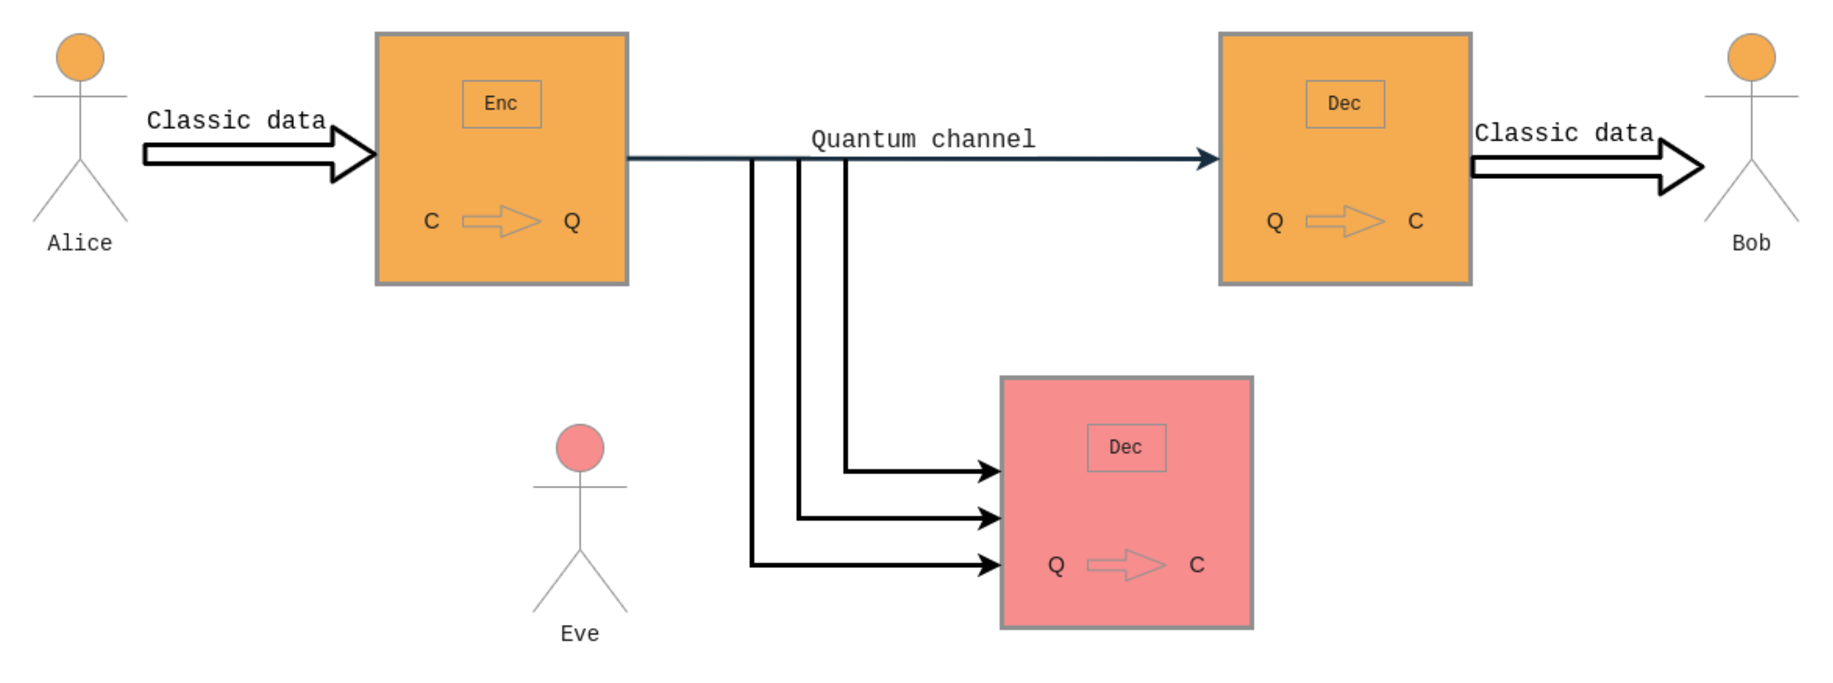
\includegraphics[width=0.8\textwidth]{figure/collective_attack.eps} 
%\end{center}
%\caption[Schema attacco coerente]{Schema che descrive un attacco coerente mostrando come Eve, oltre alla misura collettiva pu\`o ottenere informazioni dalle correlazione tra pi\`u stati.} \label{fig:attacco-coerente}
%\end{figure}
\end{itemize} 

Tornando al motivo per cui effettivamente si riesce a rilevare Eve possiamo, anche questa volta, dare il merito ai principi della fisica quantistica. Questo perch\`e in caso di misura da parte di Eve lo stato coerente trasmesso verr\`a alterato. Due esempi di attacchi che Eve pu\`o mettere in atto e le loro conseguenze sono: 
\begin{itemize}
\item sottrarre una parte del segnale per effettuare una misura sullo stesso, questo comporta una diminuzione di fotoni del segnale ricevuto da Bob
\item misura il segnale attraverso una misura eterodina per stimare entrambe le componenti di quadratura. Utilizzando le componenti misurate come valori medi, realizza un nuovo stato coerente che trasmette a Bob. In questo modo poich\'e vengono misurati dei valori randomici e la misura eterodina stessa introduce ulteriore rumore, la varianza degli stati coerenti ricevuti da Bob sar\`a superiore a quella originaria. 
\end{itemize} 
In entrambi i casi, un attacco da parte di Eve non va a far altro che aumentare gli effetti distruttivi del canale di trasmissione.


Tutte queste alterazioni, in fase di stima dei parametri, produrranno dei valori indesiderati come $\chi_{EB} > I_{AB}$. Questa incongruenza tra le stime e ci\`o che ci si aspettava dalla scelta dei paramettri iniziali portano a concludere che una spia si sia intromessa nella comunicazione. 

%\begin{figure}[bht] 
%\begin{center}
%\includegraphics[width=8cm]{figure/esempio-figura-1.eps} 
%\end{center}
%\caption{Schema che descrive le fasi del protocollo facendo particolare attenzione al canale quantistiche e canale classico.} 
%\end{figure}

